\documentclass[11pt,a4paper,titlepage]{article}
% À insérer en utilisant la commande 
%				% À insérer en utilisant la commande 
%				% À insérer en utilisant la commande 
%				\input{Func.tex}
\usepackage{PHQ405_TP}
\usepackage{makeidx}
\usepackage{amssymb}
\usepackage{amsfonts}
\usepackage{amsmath}
\usepackage{setspace}
%\NoAutoSpaceBeforeFDP
\usepackage{graphicx}
\usepackage{geometry}
\usepackage{wrapfig}
%\usepackage[usenames,dvipsnames]{color}
\usepackage[nice]{nicefrac}
\usepackage{mathrsfs}
%\usepackage[squaren,Gray]{SIunits}
%\usepackage[colorlinks=false,pdfborder={0 0 0}]{hyperref}
\usepackage[utf8x]{inputenc} 
%\usepackage[french]{babel} 
\usepackage[T1]{fontenc}
\usepackage{lmodern}
\usepackage{layout}
\usepackage{caption}
\usepackage{subcaption}
\usepackage{bbm}
\usepackage{enumerate}
\usepackage{color, colortbl}
\usepackage{braket}
\usepackage{dsfont}
\usepackage{float}

% SIunits
\newcommand{\ampere}{\text{A}}
\newcommand{\bell}{\text{B}}
\newcommand{\celsius}{\degree\text{C}}
\newcommand{\coulomb}{\text{C}}
\newcommand{\degree}{\,^{\circ}}
\newcommand{\farad}{\text{F}}
\newcommand{\electro}{\text{e}}
\newcommand{\gram}{\text{g}}
\newcommand{\henry}{\text{H}}
\newcommand{\hertz}{\text{Hz}}
\newcommand{\hour}{\text{h}}
\newcommand{\joule}{\text{J}}
\newcommand{\kelvin}{\text{K}}
\newcommand{\meter}{\text{m}}
\newcommand{\minute}{\text{m}}
\newcommand{\mole}{\text{mol}}
\newcommand{\newton}{\text{N}}
\newcommand{\ohm}{\Omega}
\newcommand{\pascal}{\text{Pa}}
\newcommand{\rad}{\text{rad}}
\newcommand{\second}{\text{s}}
\newcommand{\tesla}{\text{T}}
\newcommand{\torr}{\text{Torr}}
\newcommand{\volt}{\text{V}}
\newcommand{\watt}{\text{W}}

\newcommand{\tera}{\text{T}}
\newcommand{\giga}{\text{G}}
\newcommand{\mega}{\text{M}}
\newcommand{\kilo}{\text{k}}
\newcommand{\deci}{\text{d}}
\newcommand{\centi}{\text{c}}
\newcommand{\milli}{\text{m}}
\newcommand{\micro}{\mu}
\newcommand{\nano}{\text{n}}
\newcommand{\pico}{\text{p}}
\newcommand{\femto}{\text{f}}

\newcommand{\per}{\text{/}}

\newcommand{\Time}[3]{#1\hour~#2\minute~#3\second}
\newcommand{\Angle}[3]{#1^{\circ}~#2'~#3''}

\numberwithin{equation}{section}
\captionsetup{justification=centering}

\newcommand{\blankpage}{\pagenumbering{gobble}~\clearpage\pagenumbering{arabic}}

% Définition de l'environnement graphique
\newfloat{graph}{bth}{graph}
\floatname{graph}{\sc Graphique}

% Couleurs pour tableau
\definecolor{Gray}{gray}{0.8}
\newcolumntype{L}{>{\columncolor{Gray}}l}
\newcolumntype{C}{>{\columncolor{Gray}}c}
\newcolumntype{R}{>{\columncolor{Gray}}r}

% Page titre alternative
\makeatletter
\def\maketitlepage{
	\begin{titlepage}
	\begin{singlespace}
	\begin{center}
		\@author
		\vfill
		\textsc{\large \@title}
		\vfill
		pour le cours\\
		\@class
		\vfill
		présenté à\\
		\@teacher
		\vfill
		\@date
	\end{center}
	\end{singlespace}
	\end{titlepage}
}
\def\teacher#1{\def\@teacher{#1}}
\def\class#1{\def\@class{#1}}
\makeatother

\let\oldepsilon\epsilon
\let\epsilon\varepsilon
\let\varepsilon\oldepsilon

% Puces
\newcommand{\liste}[2]{\begin{enumerate}[#1] #2 \end{enumerate}}	% \item pour mettre une puce
\newcommand{\saute}[1]{\addtocounter{enumi}{#1}}
\newcommand{\subsaute}[1]{\addtocounter{enumii}{#1}}

% Équations
\newcommand{\al}[1]{\begin{align} #1 \end{align}}
\newcommand{\eq}[1]{\begin{equation} \begin{aligned} #1 \end{aligned} \end{equation}}
\newcommand{\eqn}[1]{\eq{ #1 \notag }}
\newcommand{\alc}[1]{\begin{gather} #1 \end{gather}}
\newcommand{\sys}[1]{\left\lbrace\begin{matrix} #1 \end{matrix}\right.}
\newcommand{\eqc}[1]{\eq{\begin{matrix} #1 \end{matrix}}}

% Maths de base
\newcommand{\Exp}[1]{\text{e}^{#1}}		% e^#
\newcommand{\p}[1]{\left( #1 \right)}	% (#)
\newcommand{\cro}[1]{\left[ #1 \right]}	% [#]
\newcommand{\norm}[1]{\left| #1\right|}	% |#|
\newcommand{\ee}[1]{\times 10^{#1}}		% X 10^#
\newcommand{\Expi}[1]{\Exp{i\p{#1}}}	% e^i(#)
\newcommand{\Expmi}[1]{\Exp{-i\p{#1}}}	% e^-i(#)
\newcommand{\avg}[1]{\left\langle #1 \right\rangle} % <#>
\newcommand{\acc}[1]{\left\lbrace #1 \right\rbrace} % {#}

% Vecteurs
\newcommand{\ve}[1]{\mathbf{#1}}
\newcommand{\vu}[1]{\hat{\ve{#1}}}
\newcommand{\vue}[1]{\vu{e}_{#1}}
\newcommand{\Ve}[1]{\overrightarrow{#1}}
\newcommand{\scal}{\cdot}
\newcommand{\vecto}{\wedge}
\newcommand{\Rot}{\Ve \nabla \times}
\newcommand{\Div}{\Ve \nabla \cdot}
\newcommand{\gve}[1]{\boldsymbol{#1}}
\newcommand{\gvu}[1]{\hat{\gve{#1}}}
\newcommand{\tens}{\otimes}
\newcommand{\sumdir}{\oplus}

% Matrices
\newcommand{\mat}[1]{\begin{pmatrix} #1 \end{pmatrix}}
\newcommand{\deter}[1]{\norm{\begin{matrix} #1 \end{matrix}}}
\newcommand{\ident}{\mathds{1}}

\newcommand{\chffk}[3]{\genfrac{[}{]}{0pt}{0}{#1~~#2}{#3}}
\newcommand{\chfsk}[3]{\genfrac{\lbrace}{\rbrace}{0pt}{0}{#1~~#2}{#3}}

% Dérivées
\newcommand{\D}{\text{d}}
\newcommand{\dd}[2]{\frac{\D#1}{\D#2}}
\newcommand{\ddn}[3]{\frac{\D^{#1}#2}{\D #3^{#1}}}
\newcommand{\dx}[1]{\dd{#1}{x}}
\newcommand{\dy}[1]{\dd{#1}{y}}
\newcommand{\dt}[1]{\dd{#1}{t}}
\newcommand{\del}{\partial}
\newcommand{\ddp}[2]{\frac{\del#1}{\del#2}}
\newcommand{\ddpn}[3]{\frac{\del^{#1}#2}{\del #3^{#1}}}

\newcommand{\eval}[1]{\left. {#1} \right|}

% Operateurs
\DeclareMathOperator{\sinc}{sinc}
\DeclareMathOperator{\sgn}{sgn}
\DeclareMathOperator{\Tr}{Tr}

% Symboles
\newcommand{\N}{\mathbbm{N}}	% nombres naturels
\newcommand{\Z}{\mathbbm{Z}}	% nombres entiers
\newcommand{\R}{\mathbbm{R}}	% nombres reels
\newcommand{\C}{\mathbbm{C}}	% nombres complexes
\newcommand{\script}[1]{\mathscr{#1}}

% Constantes
\newcommand{\eo}{\epsilon_0}

% Références
\newcommand{\US}{Université de Sherbrooke}
\newcommand{\DP}{Département de physique}
\newcommand{\dep}{département de physique}
\newcommand{\jf}{Jean-François Beaudoin}

\usepackage{PHQ405_TP}
\usepackage{makeidx}
\usepackage{amssymb}
\usepackage{amsfonts}
\usepackage{amsmath}
\usepackage{setspace}
%\NoAutoSpaceBeforeFDP
\usepackage{graphicx}
\usepackage{geometry}
\usepackage{wrapfig}
%\usepackage[usenames,dvipsnames]{color}
\usepackage[nice]{nicefrac}
\usepackage{mathrsfs}
%\usepackage[squaren,Gray]{SIunits}
%\usepackage[colorlinks=false,pdfborder={0 0 0}]{hyperref}
\usepackage[utf8x]{inputenc} 
%\usepackage[french]{babel} 
\usepackage[T1]{fontenc}
\usepackage{lmodern}
\usepackage{layout}
\usepackage{caption}
\usepackage{subcaption}
\usepackage{bbm}
\usepackage{enumerate}
\usepackage{color, colortbl}
\usepackage{braket}
\usepackage{dsfont}
\usepackage{float}

% SIunits
\newcommand{\ampere}{\text{A}}
\newcommand{\bell}{\text{B}}
\newcommand{\celsius}{\degree\text{C}}
\newcommand{\coulomb}{\text{C}}
\newcommand{\degree}{\,^{\circ}}
\newcommand{\farad}{\text{F}}
\newcommand{\electro}{\text{e}}
\newcommand{\gram}{\text{g}}
\newcommand{\henry}{\text{H}}
\newcommand{\hertz}{\text{Hz}}
\newcommand{\hour}{\text{h}}
\newcommand{\joule}{\text{J}}
\newcommand{\kelvin}{\text{K}}
\newcommand{\meter}{\text{m}}
\newcommand{\minute}{\text{m}}
\newcommand{\mole}{\text{mol}}
\newcommand{\newton}{\text{N}}
\newcommand{\ohm}{\Omega}
\newcommand{\pascal}{\text{Pa}}
\newcommand{\rad}{\text{rad}}
\newcommand{\second}{\text{s}}
\newcommand{\tesla}{\text{T}}
\newcommand{\torr}{\text{Torr}}
\newcommand{\volt}{\text{V}}
\newcommand{\watt}{\text{W}}

\newcommand{\tera}{\text{T}}
\newcommand{\giga}{\text{G}}
\newcommand{\mega}{\text{M}}
\newcommand{\kilo}{\text{k}}
\newcommand{\deci}{\text{d}}
\newcommand{\centi}{\text{c}}
\newcommand{\milli}{\text{m}}
\newcommand{\micro}{\mu}
\newcommand{\nano}{\text{n}}
\newcommand{\pico}{\text{p}}
\newcommand{\femto}{\text{f}}

\newcommand{\per}{\text{/}}

\newcommand{\Time}[3]{#1\hour~#2\minute~#3\second}
\newcommand{\Angle}[3]{#1^{\circ}~#2'~#3''}

\numberwithin{equation}{section}
\captionsetup{justification=centering}

\newcommand{\blankpage}{\pagenumbering{gobble}~\clearpage\pagenumbering{arabic}}

% Définition de l'environnement graphique
\newfloat{graph}{bth}{graph}
\floatname{graph}{\sc Graphique}

% Couleurs pour tableau
\definecolor{Gray}{gray}{0.8}
\newcolumntype{L}{>{\columncolor{Gray}}l}
\newcolumntype{C}{>{\columncolor{Gray}}c}
\newcolumntype{R}{>{\columncolor{Gray}}r}

% Page titre alternative
\makeatletter
\def\maketitlepage{
	\begin{titlepage}
	\begin{singlespace}
	\begin{center}
		\@author
		\vfill
		\textsc{\large \@title}
		\vfill
		pour le cours\\
		\@class
		\vfill
		présenté à\\
		\@teacher
		\vfill
		\@date
	\end{center}
	\end{singlespace}
	\end{titlepage}
}
\def\teacher#1{\def\@teacher{#1}}
\def\class#1{\def\@class{#1}}
\makeatother

\let\oldepsilon\epsilon
\let\epsilon\varepsilon
\let\varepsilon\oldepsilon

% Puces
\newcommand{\liste}[2]{\begin{enumerate}[#1] #2 \end{enumerate}}	% \item pour mettre une puce
\newcommand{\saute}[1]{\addtocounter{enumi}{#1}}
\newcommand{\subsaute}[1]{\addtocounter{enumii}{#1}}

% Équations
\newcommand{\al}[1]{\begin{align} #1 \end{align}}
\newcommand{\eq}[1]{\begin{equation} \begin{aligned} #1 \end{aligned} \end{equation}}
\newcommand{\eqn}[1]{\eq{ #1 \notag }}
\newcommand{\alc}[1]{\begin{gather} #1 \end{gather}}
\newcommand{\sys}[1]{\left\lbrace\begin{matrix} #1 \end{matrix}\right.}
\newcommand{\eqc}[1]{\eq{\begin{matrix} #1 \end{matrix}}}

% Maths de base
\newcommand{\Exp}[1]{\text{e}^{#1}}		% e^#
\newcommand{\p}[1]{\left( #1 \right)}	% (#)
\newcommand{\cro}[1]{\left[ #1 \right]}	% [#]
\newcommand{\norm}[1]{\left| #1\right|}	% |#|
\newcommand{\ee}[1]{\times 10^{#1}}		% X 10^#
\newcommand{\Expi}[1]{\Exp{i\p{#1}}}	% e^i(#)
\newcommand{\Expmi}[1]{\Exp{-i\p{#1}}}	% e^-i(#)
\newcommand{\avg}[1]{\left\langle #1 \right\rangle} % <#>
\newcommand{\acc}[1]{\left\lbrace #1 \right\rbrace} % {#}

% Vecteurs
\newcommand{\ve}[1]{\mathbf{#1}}
\newcommand{\vu}[1]{\hat{\ve{#1}}}
\newcommand{\vue}[1]{\vu{e}_{#1}}
\newcommand{\Ve}[1]{\overrightarrow{#1}}
\newcommand{\scal}{\cdot}
\newcommand{\vecto}{\wedge}
\newcommand{\Rot}{\Ve \nabla \times}
\newcommand{\Div}{\Ve \nabla \cdot}
\newcommand{\gve}[1]{\boldsymbol{#1}}
\newcommand{\gvu}[1]{\hat{\gve{#1}}}
\newcommand{\tens}{\otimes}
\newcommand{\sumdir}{\oplus}

% Matrices
\newcommand{\mat}[1]{\begin{pmatrix} #1 \end{pmatrix}}
\newcommand{\deter}[1]{\norm{\begin{matrix} #1 \end{matrix}}}
\newcommand{\ident}{\mathds{1}}

\newcommand{\chffk}[3]{\genfrac{[}{]}{0pt}{0}{#1~~#2}{#3}}
\newcommand{\chfsk}[3]{\genfrac{\lbrace}{\rbrace}{0pt}{0}{#1~~#2}{#3}}

% Dérivées
\newcommand{\D}{\text{d}}
\newcommand{\dd}[2]{\frac{\D#1}{\D#2}}
\newcommand{\ddn}[3]{\frac{\D^{#1}#2}{\D #3^{#1}}}
\newcommand{\dx}[1]{\dd{#1}{x}}
\newcommand{\dy}[1]{\dd{#1}{y}}
\newcommand{\dt}[1]{\dd{#1}{t}}
\newcommand{\del}{\partial}
\newcommand{\ddp}[2]{\frac{\del#1}{\del#2}}
\newcommand{\ddpn}[3]{\frac{\del^{#1}#2}{\del #3^{#1}}}

\newcommand{\eval}[1]{\left. {#1} \right|}

% Operateurs
\DeclareMathOperator{\sinc}{sinc}
\DeclareMathOperator{\sgn}{sgn}
\DeclareMathOperator{\Tr}{Tr}

% Symboles
\newcommand{\N}{\mathbbm{N}}	% nombres naturels
\newcommand{\Z}{\mathbbm{Z}}	% nombres entiers
\newcommand{\R}{\mathbbm{R}}	% nombres reels
\newcommand{\C}{\mathbbm{C}}	% nombres complexes
\newcommand{\script}[1]{\mathscr{#1}}

% Constantes
\newcommand{\eo}{\epsilon_0}

% Références
\newcommand{\US}{Université de Sherbrooke}
\newcommand{\DP}{Département de physique}
\newcommand{\dep}{département de physique}
\newcommand{\jf}{Jean-François Beaudoin}

\usepackage{PHQ405_TP}
\usepackage{makeidx}
\usepackage{amssymb}
\usepackage{amsfonts}
\usepackage{amsmath}
\usepackage{setspace}
%\NoAutoSpaceBeforeFDP
\usepackage{graphicx}
\usepackage{geometry}
\usepackage{wrapfig}
%\usepackage[usenames,dvipsnames]{color}
\usepackage[nice]{nicefrac}
\usepackage{mathrsfs}
%\usepackage[squaren,Gray]{SIunits}
%\usepackage[colorlinks=false,pdfborder={0 0 0}]{hyperref}
\usepackage[utf8x]{inputenc} 
%\usepackage[french]{babel} 
\usepackage[T1]{fontenc}
\usepackage{lmodern}
\usepackage{layout}
\usepackage{caption}
\usepackage{subcaption}
\usepackage{bbm}
\usepackage{enumerate}
\usepackage{color, colortbl}
\usepackage{braket}
\usepackage{dsfont}
\usepackage{float}

% SIunits
\newcommand{\ampere}{\text{A}}
\newcommand{\bell}{\text{B}}
\newcommand{\celsius}{\degree\text{C}}
\newcommand{\coulomb}{\text{C}}
\newcommand{\degree}{\,^{\circ}}
\newcommand{\farad}{\text{F}}
\newcommand{\electro}{\text{e}}
\newcommand{\gram}{\text{g}}
\newcommand{\henry}{\text{H}}
\newcommand{\hertz}{\text{Hz}}
\newcommand{\hour}{\text{h}}
\newcommand{\joule}{\text{J}}
\newcommand{\kelvin}{\text{K}}
\newcommand{\meter}{\text{m}}
\newcommand{\minute}{\text{m}}
\newcommand{\mole}{\text{mol}}
\newcommand{\newton}{\text{N}}
\newcommand{\ohm}{\Omega}
\newcommand{\pascal}{\text{Pa}}
\newcommand{\rad}{\text{rad}}
\newcommand{\second}{\text{s}}
\newcommand{\tesla}{\text{T}}
\newcommand{\torr}{\text{Torr}}
\newcommand{\volt}{\text{V}}
\newcommand{\watt}{\text{W}}

\newcommand{\tera}{\text{T}}
\newcommand{\giga}{\text{G}}
\newcommand{\mega}{\text{M}}
\newcommand{\kilo}{\text{k}}
\newcommand{\deci}{\text{d}}
\newcommand{\centi}{\text{c}}
\newcommand{\milli}{\text{m}}
\newcommand{\micro}{\mu}
\newcommand{\nano}{\text{n}}
\newcommand{\pico}{\text{p}}
\newcommand{\femto}{\text{f}}

\newcommand{\per}{\text{/}}

\newcommand{\Time}[3]{#1\hour~#2\minute~#3\second}
\newcommand{\Angle}[3]{#1^{\circ}~#2'~#3''}

\numberwithin{equation}{section}
\captionsetup{justification=centering}

\newcommand{\blankpage}{\pagenumbering{gobble}~\clearpage\pagenumbering{arabic}}

% Définition de l'environnement graphique
\newfloat{graph}{bth}{graph}
\floatname{graph}{\sc Graphique}

% Couleurs pour tableau
\definecolor{Gray}{gray}{0.8}
\newcolumntype{L}{>{\columncolor{Gray}}l}
\newcolumntype{C}{>{\columncolor{Gray}}c}
\newcolumntype{R}{>{\columncolor{Gray}}r}

% Page titre alternative
\makeatletter
\def\maketitlepage{
	\begin{titlepage}
	\begin{singlespace}
	\begin{center}
		\@author
		\vfill
		\textsc{\large \@title}
		\vfill
		pour le cours\\
		\@class
		\vfill
		présenté à\\
		\@teacher
		\vfill
		\@date
	\end{center}
	\end{singlespace}
	\end{titlepage}
}
\def\teacher#1{\def\@teacher{#1}}
\def\class#1{\def\@class{#1}}
\makeatother

\let\oldepsilon\epsilon
\let\epsilon\varepsilon
\let\varepsilon\oldepsilon

% Puces
\newcommand{\liste}[2]{\begin{enumerate}[#1] #2 \end{enumerate}}	% \item pour mettre une puce
\newcommand{\saute}[1]{\addtocounter{enumi}{#1}}
\newcommand{\subsaute}[1]{\addtocounter{enumii}{#1}}

% Équations
\newcommand{\al}[1]{\begin{align} #1 \end{align}}
\newcommand{\eq}[1]{\begin{equation} \begin{aligned} #1 \end{aligned} \end{equation}}
\newcommand{\eqn}[1]{\eq{ #1 \notag }}
\newcommand{\alc}[1]{\begin{gather} #1 \end{gather}}
\newcommand{\sys}[1]{\left\lbrace\begin{matrix} #1 \end{matrix}\right.}
\newcommand{\eqc}[1]{\eq{\begin{matrix} #1 \end{matrix}}}

% Maths de base
\newcommand{\Exp}[1]{\text{e}^{#1}}		% e^#
\newcommand{\p}[1]{\left( #1 \right)}	% (#)
\newcommand{\cro}[1]{\left[ #1 \right]}	% [#]
\newcommand{\norm}[1]{\left| #1\right|}	% |#|
\newcommand{\ee}[1]{\times 10^{#1}}		% X 10^#
\newcommand{\Expi}[1]{\Exp{i\p{#1}}}	% e^i(#)
\newcommand{\Expmi}[1]{\Exp{-i\p{#1}}}	% e^-i(#)
\newcommand{\avg}[1]{\left\langle #1 \right\rangle} % <#>
\newcommand{\acc}[1]{\left\lbrace #1 \right\rbrace} % {#}

% Vecteurs
\newcommand{\ve}[1]{\mathbf{#1}}
\newcommand{\vu}[1]{\hat{\ve{#1}}}
\newcommand{\vue}[1]{\vu{e}_{#1}}
\newcommand{\Ve}[1]{\overrightarrow{#1}}
\newcommand{\scal}{\cdot}
\newcommand{\vecto}{\wedge}
\newcommand{\Rot}{\Ve \nabla \times}
\newcommand{\Div}{\Ve \nabla \cdot}
\newcommand{\gve}[1]{\boldsymbol{#1}}
\newcommand{\gvu}[1]{\hat{\gve{#1}}}
\newcommand{\tens}{\otimes}
\newcommand{\sumdir}{\oplus}

% Matrices
\newcommand{\mat}[1]{\begin{pmatrix} #1 \end{pmatrix}}
\newcommand{\deter}[1]{\norm{\begin{matrix} #1 \end{matrix}}}
\newcommand{\ident}{\mathds{1}}

\newcommand{\chffk}[3]{\genfrac{[}{]}{0pt}{0}{#1~~#2}{#3}}
\newcommand{\chfsk}[3]{\genfrac{\lbrace}{\rbrace}{0pt}{0}{#1~~#2}{#3}}

% Dérivées
\newcommand{\D}{\text{d}}
\newcommand{\dd}[2]{\frac{\D#1}{\D#2}}
\newcommand{\ddn}[3]{\frac{\D^{#1}#2}{\D #3^{#1}}}
\newcommand{\dx}[1]{\dd{#1}{x}}
\newcommand{\dy}[1]{\dd{#1}{y}}
\newcommand{\dt}[1]{\dd{#1}{t}}
\newcommand{\del}{\partial}
\newcommand{\ddp}[2]{\frac{\del#1}{\del#2}}
\newcommand{\ddpn}[3]{\frac{\del^{#1}#2}{\del #3^{#1}}}

\newcommand{\eval}[1]{\left. {#1} \right|}

% Operateurs
\DeclareMathOperator{\sinc}{sinc}
\DeclareMathOperator{\sgn}{sgn}
\DeclareMathOperator{\Tr}{Tr}

% Symboles
\newcommand{\N}{\mathbbm{N}}	% nombres naturels
\newcommand{\Z}{\mathbbm{Z}}	% nombres entiers
\newcommand{\R}{\mathbbm{R}}	% nombres reels
\newcommand{\C}{\mathbbm{C}}	% nombres complexes
\newcommand{\script}[1]{\mathscr{#1}}

% Constantes
\newcommand{\eo}{\epsilon_0}

% Références
\newcommand{\US}{Université de Sherbrooke}
\newcommand{\DP}{Département de physique}
\newcommand{\dep}{département de physique}
\newcommand{\jf}{Jean-François Beaudoin}

\graphicspath {{.}/{fig}}
\begin{document}

\author{\jf}
\title{Devoir 3}
\teacher{Louis-Philippe Nadeau}
\class{Analyse en océanographie physique}
\date{Ismer \\ UQAR \\ \today}
\onehalfspacing
\setlength{\parindent}{0cm}
\renewcommand\thesection{\arabic{section}}
\renewcommand\thesubsection{\thesection.\arabic{subsection}}

\maketitlepage

\blankpage

\section{}

Les équations d'Ekman pour $V_e$ à $U_e$ sont:

\begin{equation}
-f V_e = A \del_{zz} U_e
 \label{1}
\end{equation}
\begin{equation}
f U_e = A \del_{zz} V_e.
\end{equation}

À partir de l'équation \label{1} il est possible de trouver directement la solution générale de $V_e$ en dérivant deux fois la solution générale de $U_e$. La solution générale de $V_e$ est alors:

\begin{equation}
V_e = \frac{-A}{f} Re \left[C_1 \frac{(1+i)^2}{\delta_e^2}e^{\frac{(1+i)z}{\delta_e}}+C_2 \frac{(1-i)^2}{\delta_e^2}e^{\frac{(1-i)z}{\delta_e}}+C_3 \frac{-(1+i)^2}{\delta_e^2}e^{\frac{-(1+i)z}{\delta_e}}+C_4 \frac{-(1-i)^2}{\delta_e^2}e^{\frac{-(1-i)z}{\delta_e}}\right] \nonumber
\end{equation}

\begin{equation}
\Rightarrow V_e = \frac{-A}{f} Re \left[\frac{2i}{\delta_e^2}\left[ C_1 e^{\frac{(1+i)z}{\delta_e}}-C_2 e^{\frac{(1-i)z}{\delta_e}}+C_3 e^{\frac{-(1+i)z}{\delta_e}}-C_4 e^{\frac{-(1-i)z}{\delta_e}}\right]\right] \nonumber
\end{equation}

\begin{equation}
\Rightarrow V_e =  Re \left[-i \left[C_1 e^{\frac{(1+i)z}{\delta_e}}-C_2 e^{\frac{(1-i)z}{\delta_e}}+C_3 e^{\frac{-(1+i)z}{\delta_e}}-C_4 e^{\frac{-(1-i)z}{\delta_e}}\right]\right]
\end{equation}


\subsection{}
Pour éviter que la solution diverge en haut de l'atmosphère les $C_1$ et $C_2$ de la couche d'Ekman dans l'atmosphère doivent être nulles. De même, avec un axe des z positifs vers le haut il faut que la solution dans l'océan ait des $C_3$ et $C_4$ nulles.  La solution pour les deux couches est alors: 

\textbf{Pour l'océan}
\begin{equation}
\Rightarrow U_e =  Re \left[ C_1 e^{\frac{(1+i)z}{\delta_e}}+C_2 e^{\frac{(1-i)z}{\delta_e}} \right] 
\end{equation}

\begin{equation}
\Rightarrow V_e =  Re \left[-i \left[C_1 e^{\frac{(1+i)z}{\delta_e}}-C_2 e^{\frac{(1-i)z}{\delta_e}}\right]\right]
\end{equation}

\pagebreak

textbf{Pour l'air}
\begin{equation}
\Rightarrow U_e =  Re \left[ C_3 e^{\frac{(1+i)z}{\delta_e}}+C_4 e^{\frac{(1-i)z}{\delta_e}} \right] \linebreak
\end{equation}
\begin{equation}
\Rightarrow V_e =  Re \left[-i \left[C_3 e^{\frac{(1+i)z}{\delta_e}}-C_4 e^{\frac{(1-i)z}{\delta_e}}\right]\right]
\end{equation}

À $z=0$, la conditions de continuité des vitesses oblige:

\begin{equation}
U_{go}+U_{eo} = U_{ga}+U_{ea}
\end{equation}

\begin{equation}
V_{go}+V_{eo} = V_{ga}+V_{ea}
\end{equation}

Où les indice $g$ et $e$ représentent les vitesse géostrophique et d'Ekman et les indices $o$ et $a$ représente l'océan et l'atmosphère. On a alors les deux équations ci dessous:

\begin{equation}
\begin{cases} 
C_1 + C_2 + U_{go} = C_3 + C_4 + U_{ga} \\
C_1 + C_2 + i V_{go} = C_3 + C_4 + i V_{ga} 
\end{cases}
\end{equation}

Les flux de quantité de mouvement verticaux sont donné par:
\begin{equation}
Flux^k = A \del_z U 
\end{equation}

On a donc :
\begin{equation}
A_{o} \del_z U_{eo} = A_{a} \del_z U_{ea} 
A_{o} \del_z V_{eo} = A_{a} \del_z V_{ea} 
\end{equation}

On peut remplacer $A_{o}$ et $A_{a}$ par $f/2 \delta_o^2$ et $f/2 \delta_a^2$ 

En dérivant correctement les U et V on obtient les quatres équations :

\begin{equation}
\begin{cases} 
C_1 + C_2 + U_{go} = C_3 + C_4 + U_{ga} \\
C_1 - C_2 + i V_{go} = C_3 - C_4 + i V_{ga}\\
(1+i)C_1 + (1-i) C_2 = - \dfrac{\delta_a}{\delta_o}\left[(1+i)C_3 + (1-i) C_4\right]\\ 
(1+i)C_1 - (1-i) C_2 = - \dfrac{\delta_a}{\delta_o}\left[(1+i)C_3 - (1-i) C_4\right]
\end{cases}
\end{equation}

On résout le système!!!
\pagebreak
En aditionnant et en soustrayant les deux premières et les deux dernières équations on obtient :

\begin{equation}
\begin{cases} 
2 C_1 = 2 C_3 + \Delta U_{ao} + i \Delta V_{ao} \\
2 C_2 = 2 C_4 + \Delta U_{ao} - i \Delta V_{ao} \\
C_1 = -\dfrac{\delta_a}{\delta_o}C_3 \\
C_2 = -\dfrac{\delta_a}{\delta_o} C_4
\end{cases}
\end{equation}

Avec, $\Delta U_{ao} = U_a-U_o$ et  $\Delta V_{ao}= V_a-V_o$ 
On a alors: 

\begin{equation}
C_3 \left[-2\left[\dfrac{\delta_a}{\delta_o}+1\right]\right] = \Delta U_{ao} + i \Delta V_{ao} 
\end{equation}

\begin{equation}
\Rightarrow C_3 =\dfrac{1}{\left[-2\left[\dfrac{\delta_a}{\delta_o}+1\right]\right] } (\Delta U_{ao} + i \Delta V_{ao}) 
\end{equation}

\begin{equation}
\Rightarrow C_1 =\dfrac{\delta_a}{\delta_o \left[2\left[\dfrac{\delta_a}{\delta_o}+1\right]\right] } (\Delta U_{ao} + i \Delta V_{ao}) 
\end{equation}

De façon analogue on trouve $C_2$ et $C_4$ pour obtenir:

\begin{equation}
\Rightarrow C_4 =\dfrac{1}{\left[-2\left[\dfrac{\delta_a}{\delta_o}+1\right]\right] } (\Delta U_{ao} - i \Delta V_{ao}) 
\end{equation}

\begin{equation}
\Rightarrow C_2 =\dfrac{\delta_a}{\delta_o \left[2\left[\dfrac{\delta_a}{\delta_o}+1\right]\right] } (\Delta U_{ao} -  i \Delta V_{ao})
\end{equation}

En utilisant ces définition des constantes on trouve les $U_e$ et $V_e$ pour l'océan et latmosphère.
\textbf{Pour l'océan :}
\begin{equation}
U_{eo} = Re \left[ \dfrac{\delta_a}{\delta_o \left[2\left[\dfrac{\delta_a}{\delta_o}+1\right]\right] } \Delta U_{ao} + i \Delta V_{ao}  e^{\frac{(1+i)z}{\delta_e}}+\dfrac{\delta_a}{\delta_o \left[2\left[\dfrac{\delta_a}{\delta_o}+1\right]\right] } \Delta U_{ao} -  i \Delta V_{ao} e^{\frac{(1-i)z}{\delta_e}} \right] 
\end{equation}


\begin{equation}
=  e^{\frac{z}{\delta_o}} \frac{K}{2}  \left[(\Delta U_{ao} +  i \Delta V_{ao})(\cos(z/\delta_0)+i \sin(z/\delta_0)) + (\Delta U_{ao} -  i \Delta V_{ao}) (\cos(z/\delta_0) - i \sin(z/\delta_0)) \right] 
\end{equation}
 Avec $K =  \dfrac{\delta_a}{\delta_o \left[\dfrac{\delta_a}{\delta_o}+1 \right]  }$

\begin{equation}
\Rightarrow U_{eo} =  e^{\frac{z}{\delta_o}} K (\Delta U_{ao} \cos(z/\delta_0) -\Delta V_{ao} \sin(z/\delta_0))
\end{equation}

De façon analogue on trouve:

\begin{equation}
\Rightarrow V_{eo} =   e^{\frac{z}{\delta_o}} K (\Delta U_{ao} \sin(z/\delta_0) + \Delta V_{ao} \cos(z/\delta_0))
\end{equation}

Dans l'atmosphère on trouve: 

\begin{equation}
\Rightarrow U_{ea} =  e^{\frac{z}{\delta_a}} B (- \Delta U_{ao} \cos(z/\delta_a) - \Delta V_{ao}  \sin(z/\delta_a))
\end{equation}


\begin{equation}
\Rightarrow V_{ea} =   e^{\frac{z}{\delta_a}} B (\Delta U_{ao} \sin(z/\delta_a) - \Delta V_{ao} \cos(z/\delta_a))
\end{equation}

Avec $B = \dfrac{1}{ \left[\dfrac{\delta_a}{\delta_o}+1 \right]}$

En se rappelant que les flux de quantité de mouvement sont donné par: 

\begin{equation}
Flux^k = A \del_z U 
\end{equation}

On trouve pour l'océan: 

\begin{equation}
Flux_x = \dfrac{A_o}{\delta_o} e^{\frac{z}{\delta_o}} K (\Delta U_{ao} +\Delta V_{ao}) \sin(z/\delta_0) + (\Delta U_{ao} - \Delta V_{ao}) \cos(z/\delta_0) 
\end{equation}

\begin{equation}
Flux_y = \dfrac{A_o}{\delta_o} e^{\frac{z}{\delta_o}} K (\Delta U_{ao} +\Delta V_{ao}) \cos(z/\delta_0) + (\Delta V_{ao} - \Delta U_{ao}) \sin(z/\delta_0) 
\end{equation}

\pagebreak

On trouve pour l'atmosphère: 

\begin{equation}
Flux_x = \dfrac{A_a}{\delta_a} e^{\frac{-z}{\delta_a}} B ((\Delta U_{ao} - \Delta V_{ao}  )\cos(z/\delta_a)  - (\Delta U_{ao} + \Delta V_{ao})  \sin(z/\delta_a)
\end{equation}

\begin{equation}
Flux_y = \dfrac{A_a}{\delta_a} e^{\frac{-z}{\delta_a}} B ((\Delta U_{ao} + \Delta V_{ao})  \cos(z/\delta_a)  + (\Delta U_{ao} - \Delta V_{ao})  \sin(z/\delta_a)
\end{equation}



On peut voir sur les graphiques représentant la vitesse et le flux en fonction de la hauteur comment agit le terme source dans l'équation.
Dans le cas ou les $\delta_o$ et $\delta_a$ sont églaes et que la différence des vitesse en U est de 0.5 avec pas de vitesse en V. On voit des couches d'Ekman symétriques. Dans ce cas, les vitesses et les flux ont la forme de:

\begin{figure}[H]
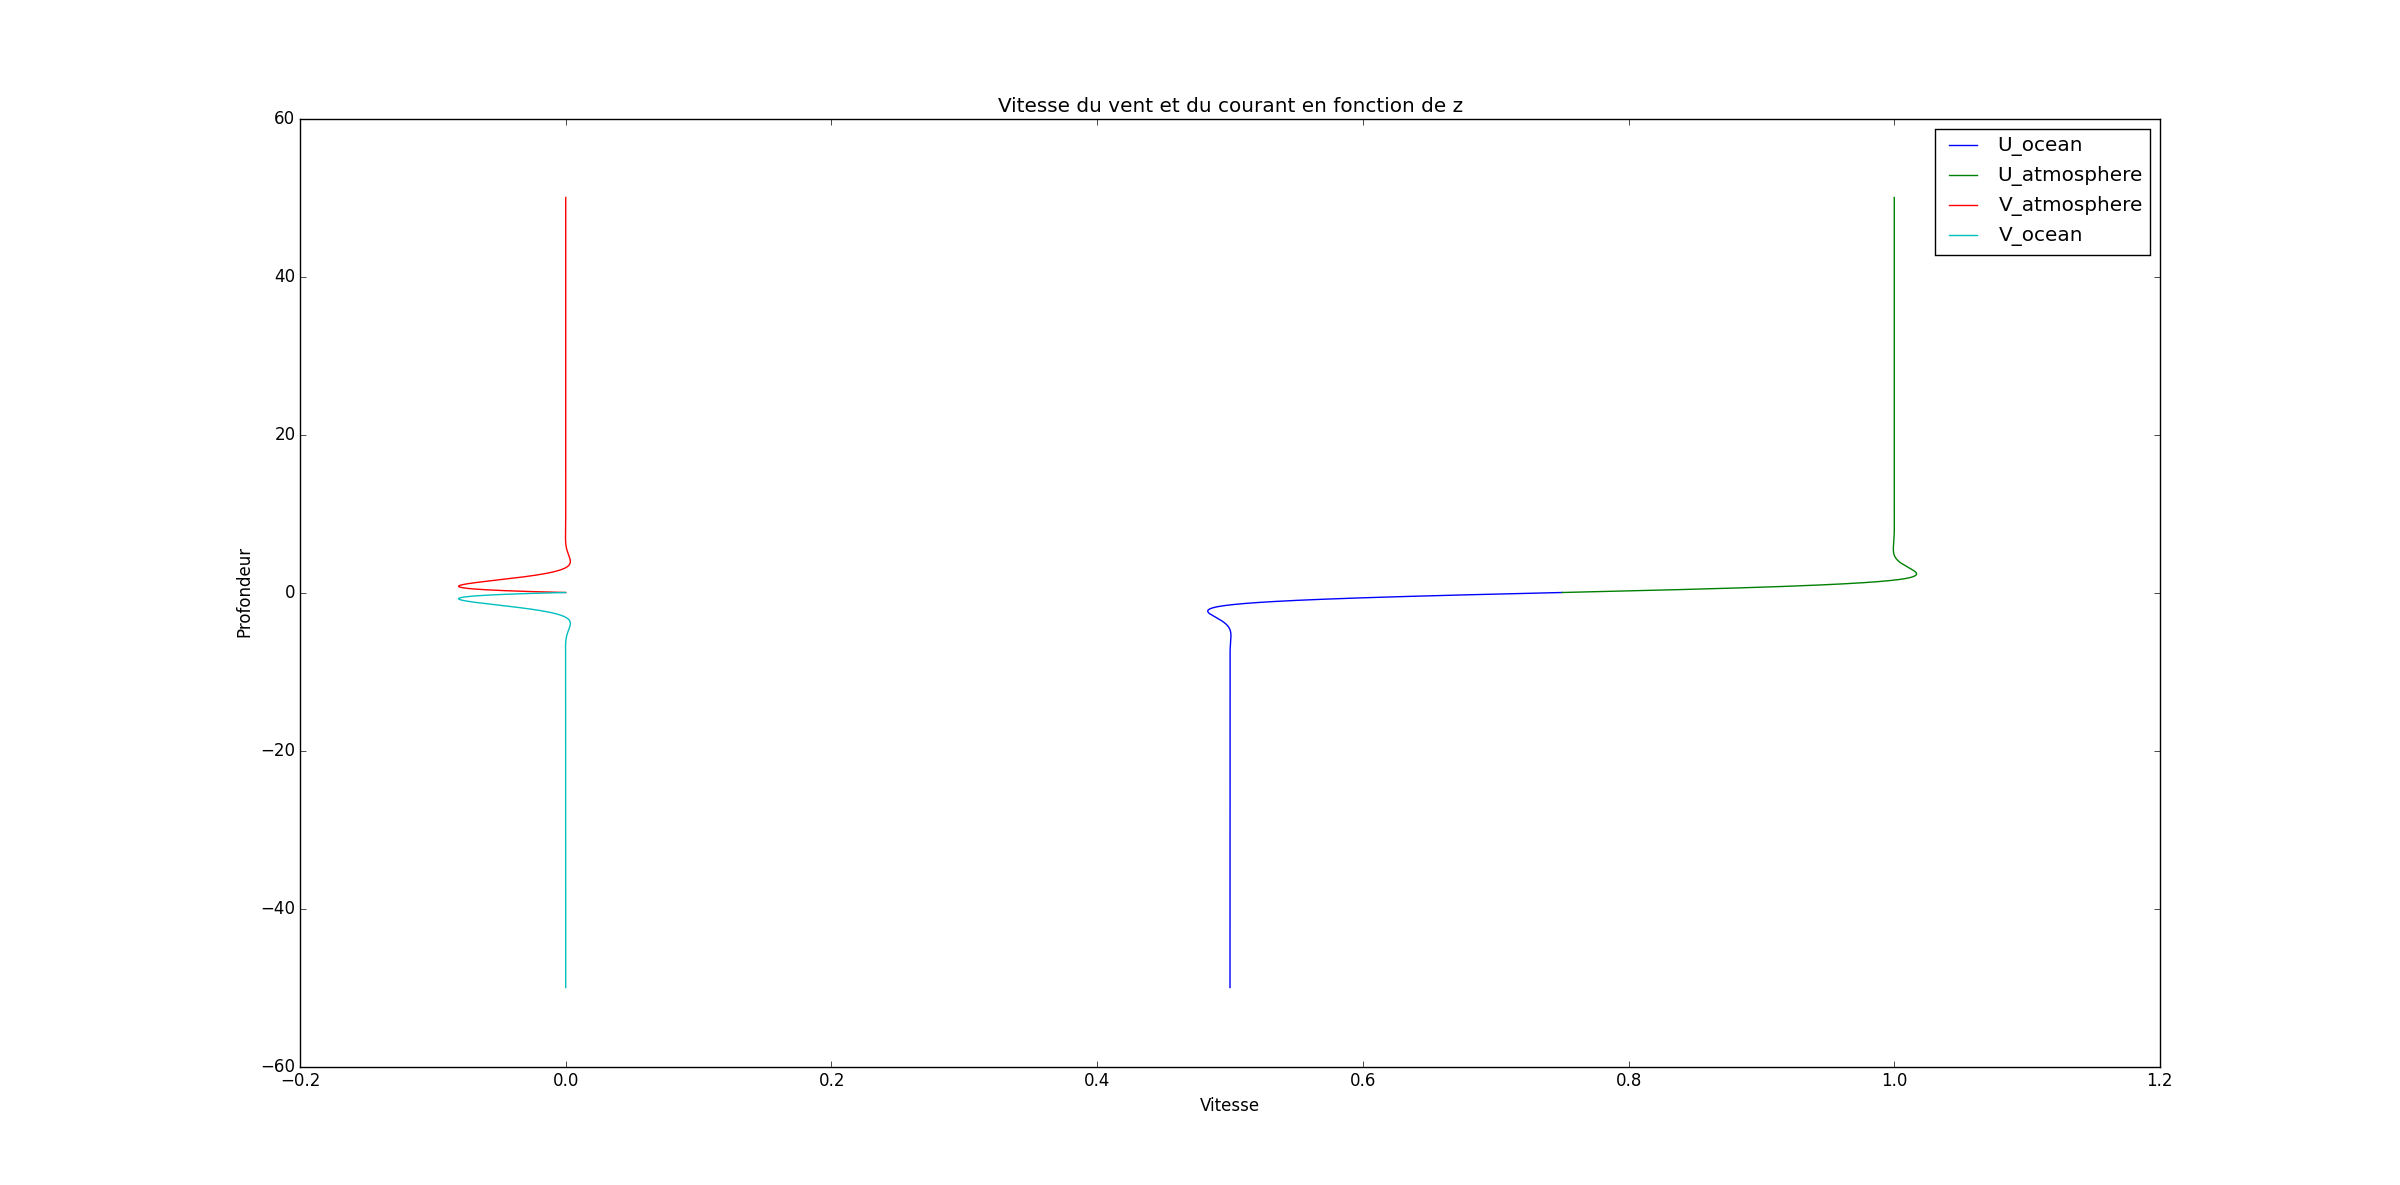
\includegraphics[width = \linewidth]{DELTAODELTAA1}
\caption{Vitesse dans la couche d'Ekman $\dfrac{\delta_a}{\delta_o}=1$, $\Delta U = 0.5$,$\Delta V = 0$ }
\end{figure}

\begin{figure}[H]
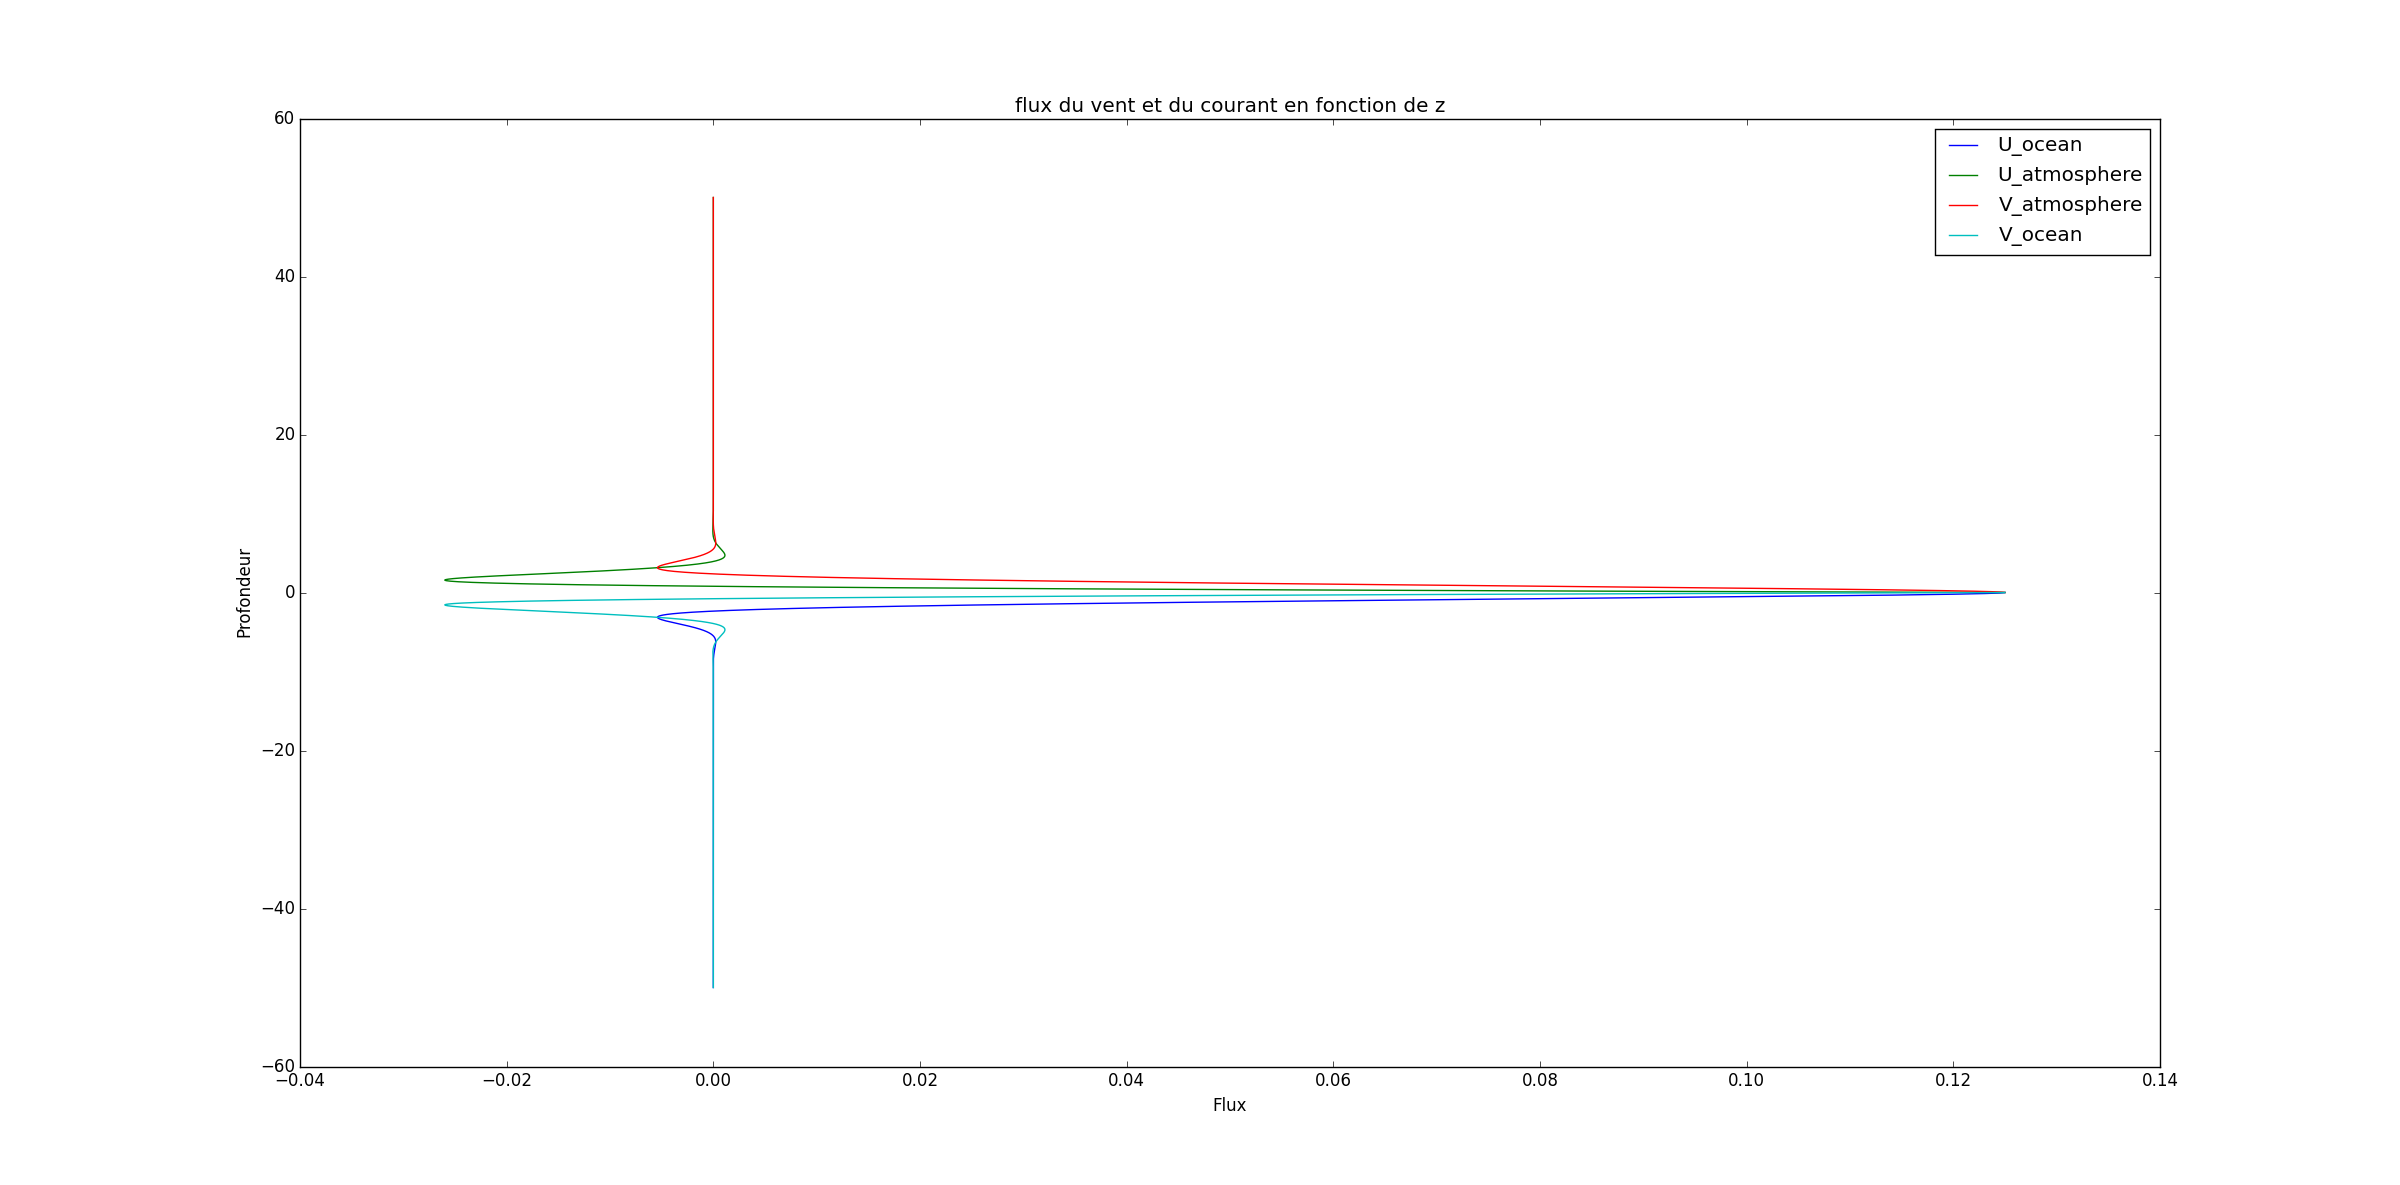
\includegraphics[width = \linewidth]{DELTAODELTAA1FLUX}
\caption{Flux dans la couche d'Ekman $\dfrac{\delta_a}{\delta_o}=1$, $\Delta U = 0.5$,$\Delta V = 0$ }
\end{figure}

En augmentant la viscosité de l'océan et donc la profondeur caractéristiques de la couche d'ekman on peut voir que les changement de vitesse de l'océan sont moins gros et que les flux de quantité vont plus profondément (fig \ref{20} et  \ref{20f}  ). La viscosité permet donc à l'eau plus profondes de ressentir directement l'effet du vent. Dans ces graphique il n'y a pas de vitesse géostrophique en V et le rapport $\delta_a/\delta_0 = 20$ 

\begin{figure}[H]
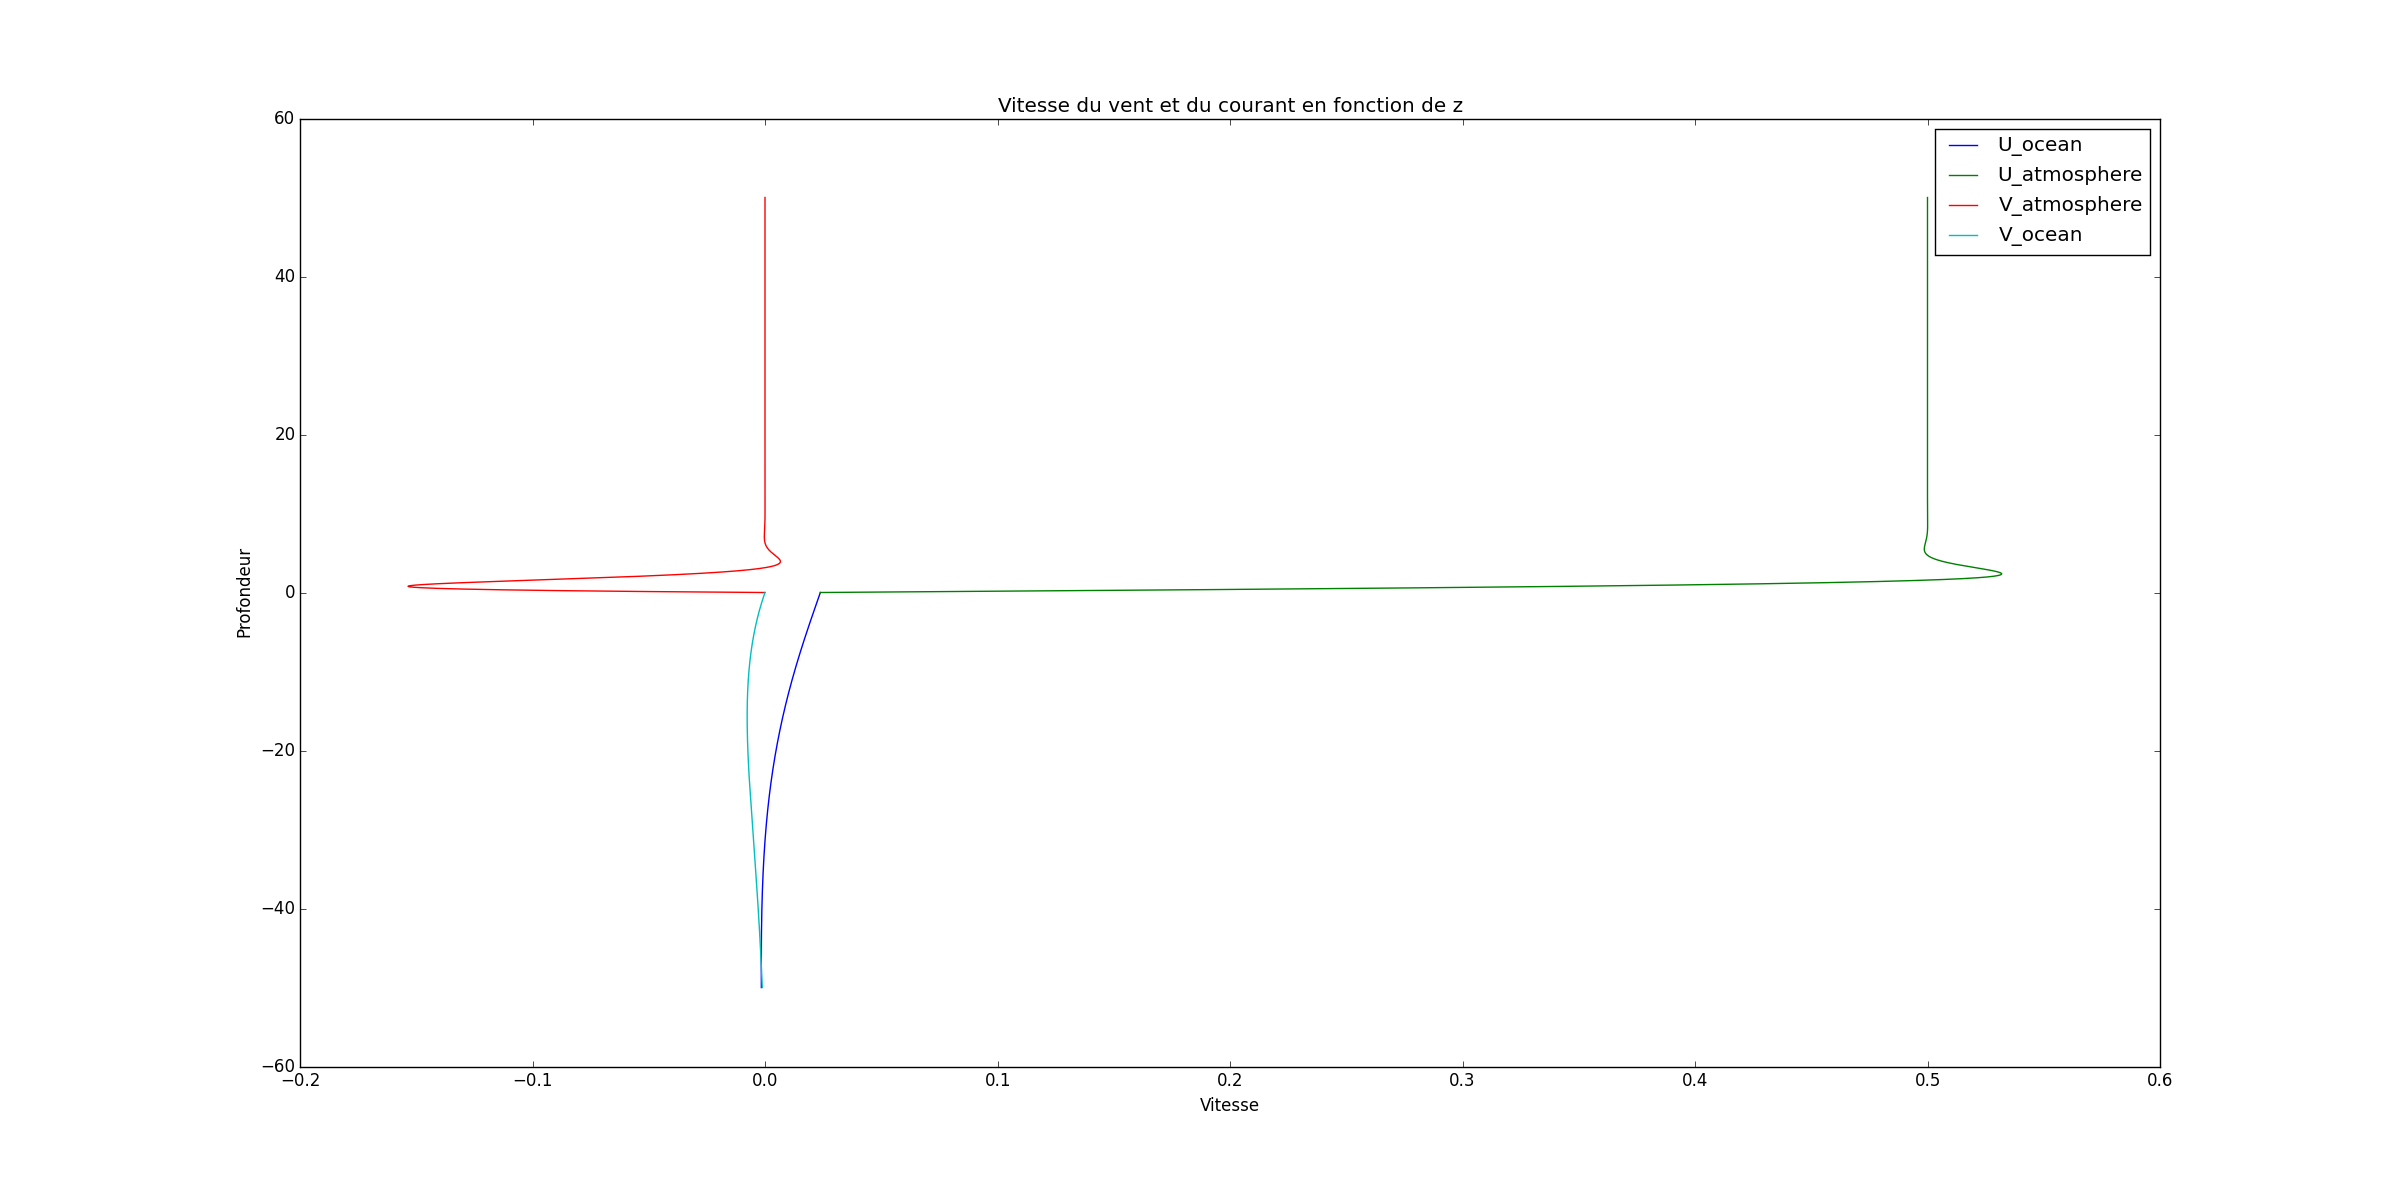
\includegraphics[width = \linewidth]{DELTAODELTAA20}
\caption{Vitesse dans la couche d'Ekman $\dfrac{\delta_a}{\delta_o}=20$, $\Delta U = 0.5$,$\Delta V = 0$}
\label{20}
\end{figure}

\begin{figure}[H]
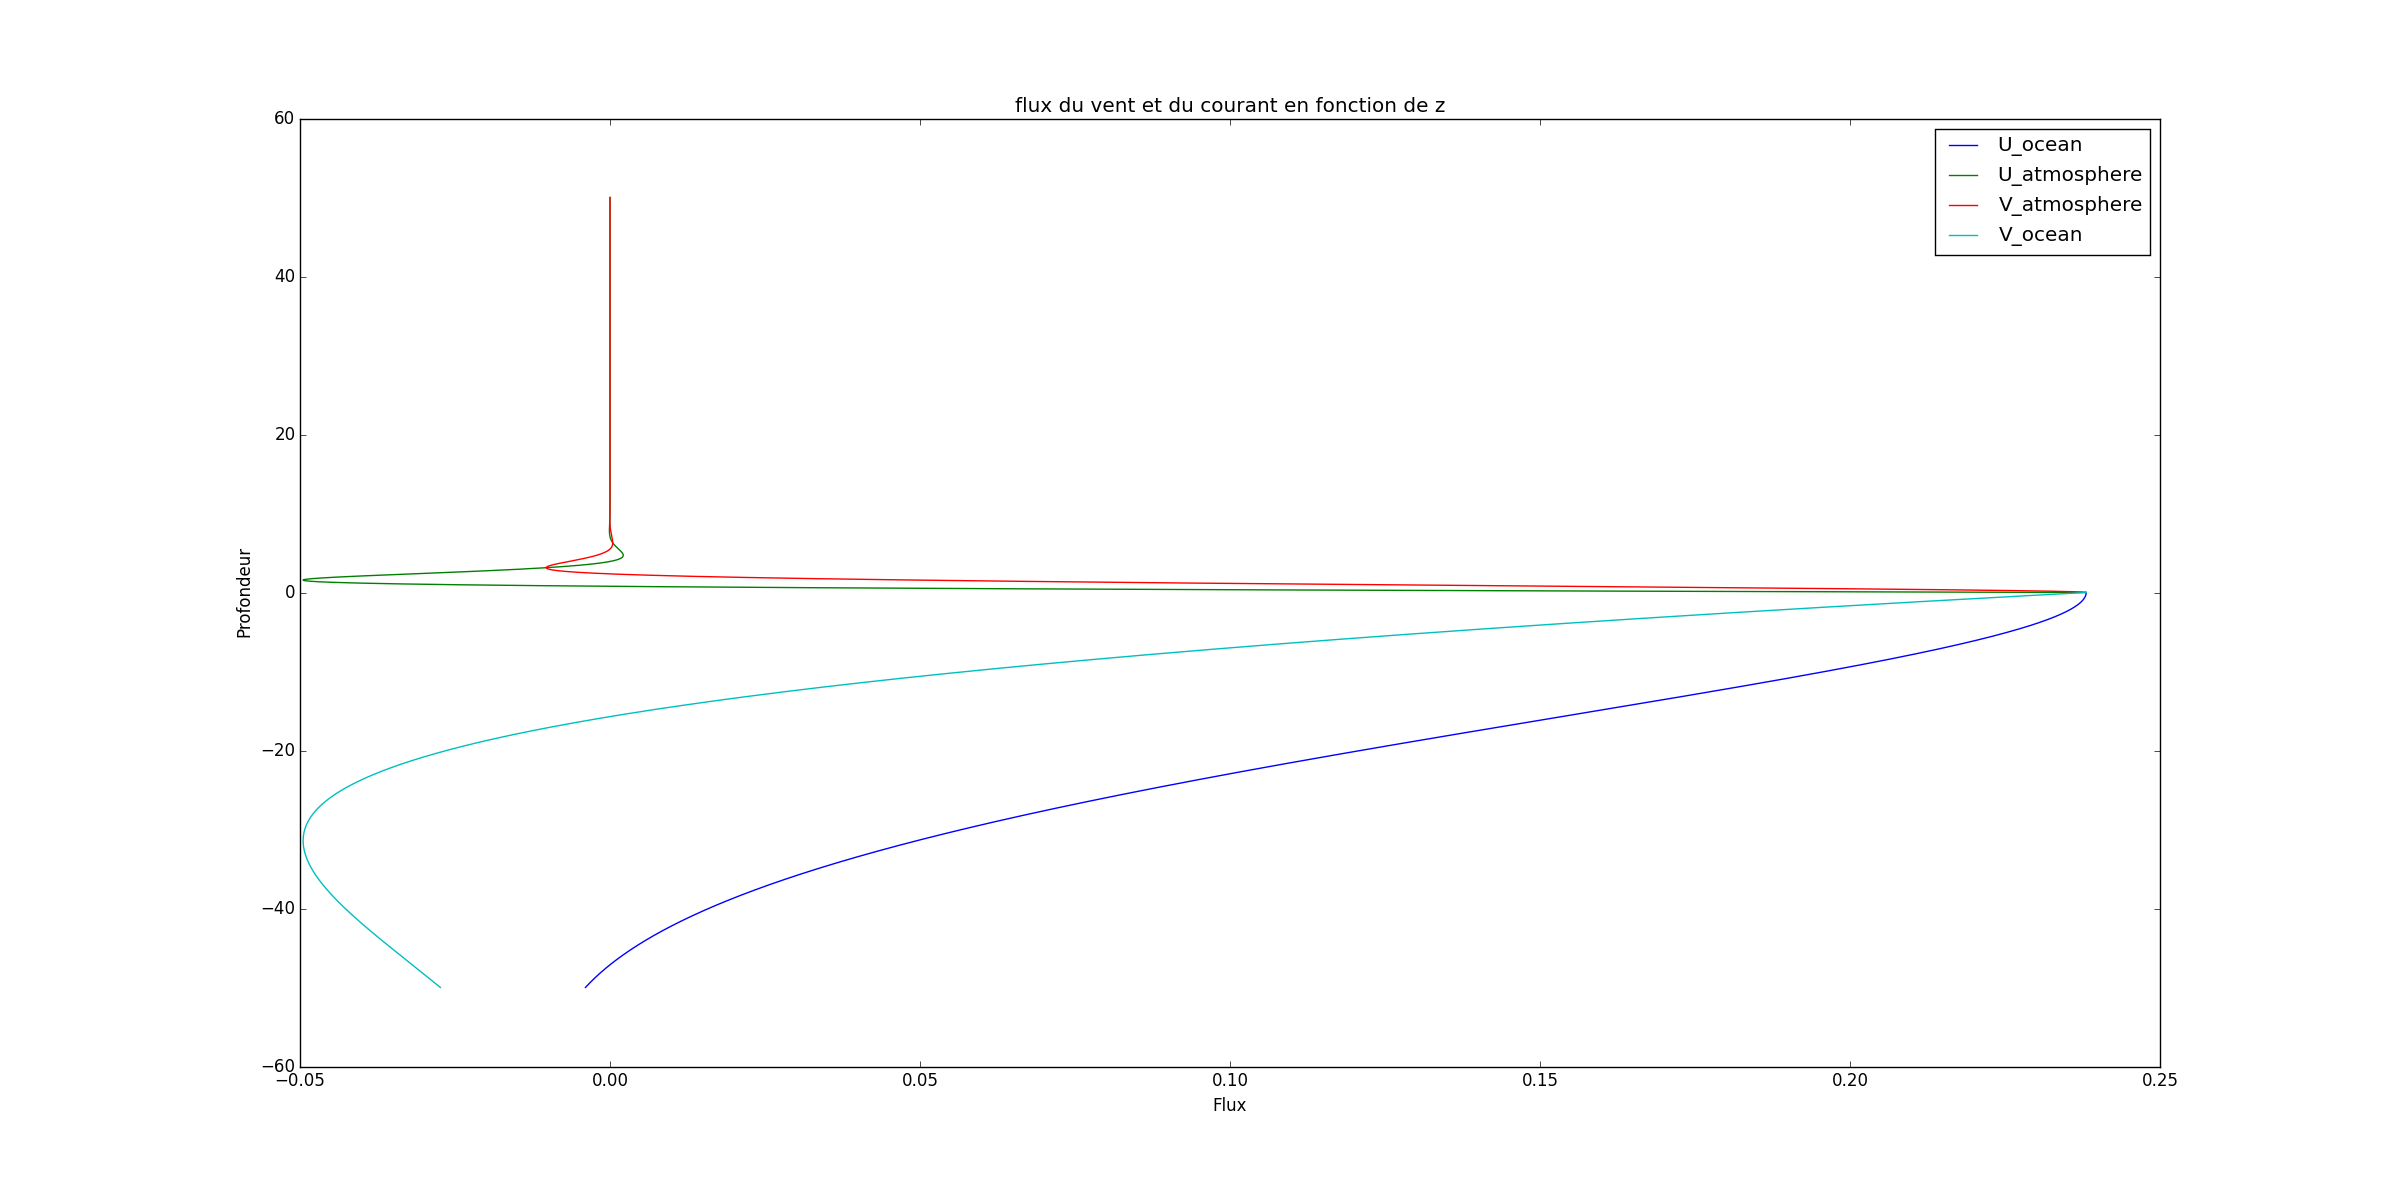
\includegraphics[width = \linewidth]{DELTAODELTAA20FLUX}
\caption{Flux dans la couche d'Ekman $\dfrac{\delta_a}{\delta_o}=20$, $\Delta U = 0.5$,$\Delta V = 0$ }
\label{20f}

\end{figure}

En augmentant encore la viscosité dans l'océan on peut voir que les changement de vitesses dans l'océan sont beaucoup plus petit. C'est une situation semblable à ce qui se passerait entre l'atmosphère et la terre.

\begin{figure}[H]
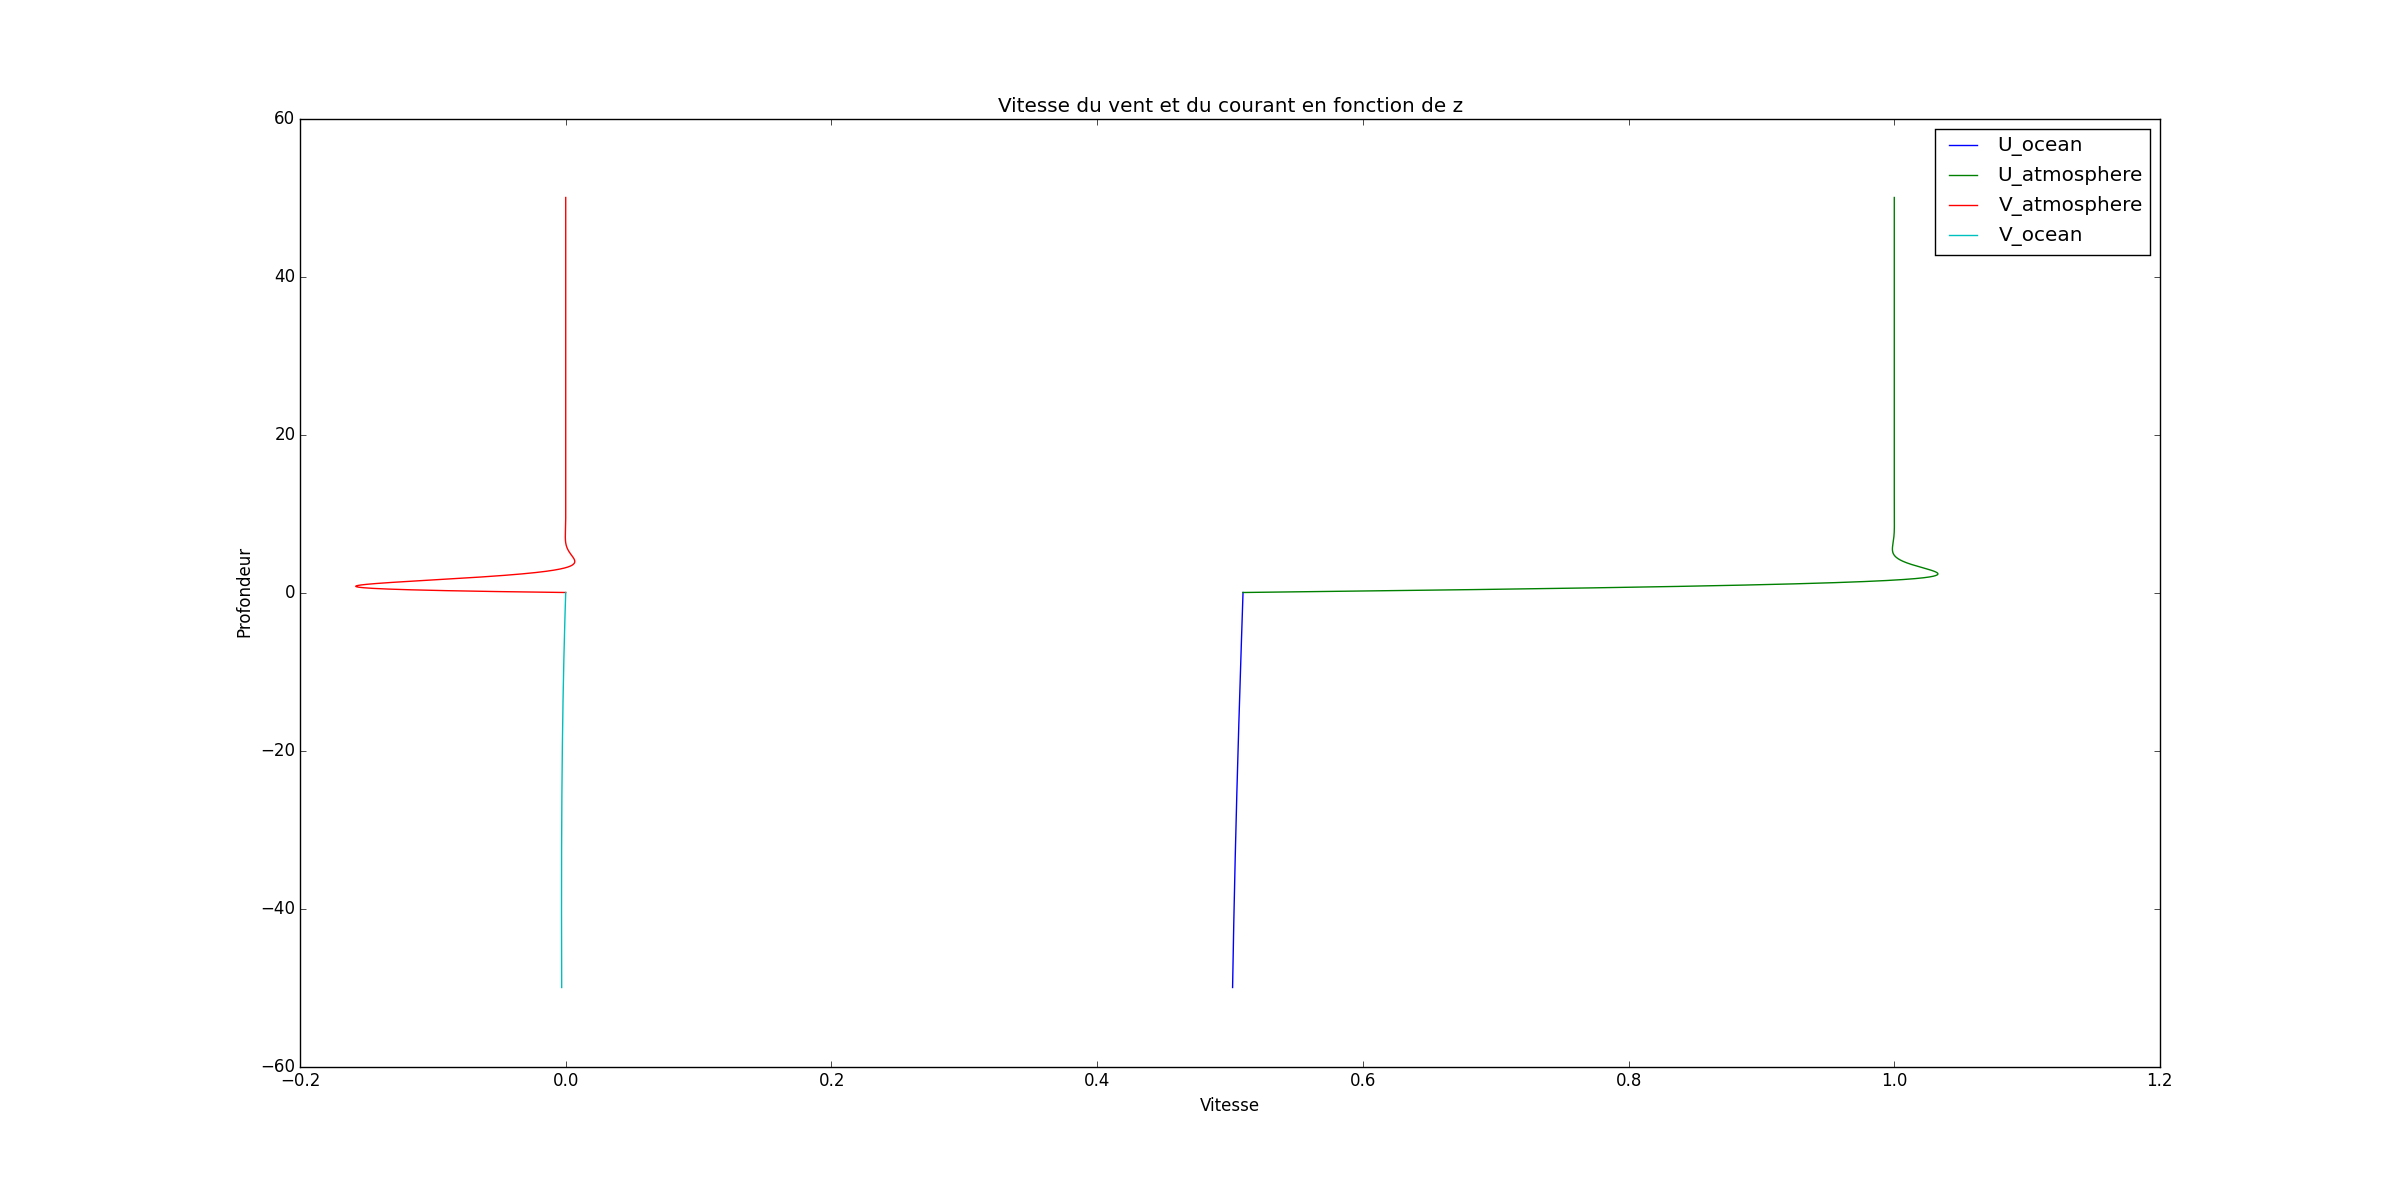
\includegraphics[width = \linewidth]{DELTAODELTAA50}
\caption{Vitesse dans la couche d'Ekman $\dfrac{\delta_a}{\delta_o}=50$, $\Delta U = 0.5$,$\Delta V = 0$}
\end{figure}

Les graphiques ne sont cependant pas réaliste car les valeurs de vitesse atmosphérique sont beaucoup plus grande que les vitesses dans l'océan ce qui n'est pas le cas ici. Par contre, les graphiques nous permettent tout de même de voir la structure de la couche d'Ekman.

\textbf{Contrainte et transport}

Pour vérifier si la contrainte et le transport sont perpendiculaires il faut intégrer les équations de vitesse et de flux sur la colonne d'eau et l'atmosphère. Techniquement, cela devrait donner des vecteurs perpendiculaires. Si on intègre de $0$ à $\infty$ les composantes des vitesses pour obtenir le transport on obtient:

\begin{equation}
 \int_{o}^{-\infty} U_{eo} = \int_{o}^{-\infty} e^{\frac{z}{\delta_o}} K (\Delta U_{ao} \cos(z/\delta_0) -\Delta V_{ao} \sin(z/\delta_0))
\end{equation}

\begin{equation}
\Rightarrow Q_{ox} =  \dfrac{-K}{2}(\Delta U_{ao} + \Delta V_{ao})
\end{equation}
De façon analogue on trouve:

\begin{equation}
\Rightarrow Q_{oy} =   \dfrac{K}{2}(\Delta U_{ao} - \Delta V_{ao})
\end{equation}

Dans l'atmosphère le transport vaut:

\begin{equation}
\Rightarrow Q_{ax} =   \dfrac{-B}{2}(\Delta U_{ao} + \Delta V_{ao})
\end{equation}

\begin{equation}
\Rightarrow Q_{ay} =   \dfrac{B}{2}(\Delta U_{ao} - \Delta V_{ao})
\end{equation}

La contrainte est quant à elle la valeur des flux à l'interface d'un côté et de l'autre multiplié par la densité.

On trouve pour l'océan: 

\begin{equation}
\tau_x = \dfrac{A_o}{\delta_o}  K (\Delta U_{ao} - \Delta V_{ao}) 
\end{equation}

\begin{equation}
\tau_y = \dfrac{A_o}{\delta_o} K (\Delta U_{ao} +\Delta V_{ao})
\end{equation}

\pagebreak

On trouve pour l'atmosphère: 

\begin{equation}
\tau_{ax} = \dfrac{A_a}{\delta_a} B (\Delta U_{ao} - \Delta V_{ao}  ) 
\end{equation}

\begin{equation}
\tau_{ay} = \dfrac{A_a}{\delta_a}  B (\Delta U_{ao} + \Delta V_{ao})
\end{equation}

Si on fait le produit scalaire entre le transport et la contrainte on obtient pour l'océan:
\begin{equation}
(\dfrac{A_o}{\delta_o}  K) \left(\dfrac{-K}{2}\right) ((\Delta U_{ao} - \Delta V_{ao})(\Delta U_{ao} + \Delta V_{ao}) )+\left(\dfrac{A_o}{\delta_o} K\right)\left(\dfrac{K}{2}\right)((\Delta U_{ao} - \Delta V_{ao})(\Delta U_{ao} +\Delta V_{ao}) = 0
\end{equation}

On trouve pour l'atmosphère: 
\begin{equation}
(\dfrac{A_a}{\delta_a}  B) \left(\dfrac{-B}{2}\right) ((\Delta U_{ao} - \Delta V_{ao})(\Delta U_{ao} + \Delta V_{ao}) )+\left(\dfrac{A_a}{\delta_a} B\right)\left(\dfrac{B}{2}\right)((\Delta U_{ao} - \Delta V_{ao})(\Delta U_{ao} +\Delta V_{ao}) = 0
\end{equation}


Les deux vecteurs sont donc perpendiculaires !!!!

\pagebreak
 
\section{}

Le critère pour obtenir de l'instabilité est d'avoir une partie imaginaire à la vitesse qui entraîne une augmentation exponentielle de l'onde. Pour cela il faut que la racine soit négative et donc que:

\begin{equation}
\dfrac{\beta^2 k_d^4}{U^2} < 4 K^4 (k_d^4-K^4)
\end{equation}

Le cisaillement minimal aura lieu lorsque $ 4 \dfrac{K^4}{k_d^4 }(k_d^4-K^4)$ sera maximal. Pour trouve le maximum il suffit de dériver et de trouver le zéro.

\begin{equation}
\dfrac{d  (4 x - \frac{x^2}{b})}{d x} = 0
\end{equation}

\begin{equation}
\Rightarrow x = \dfrac{b}{2}
\end{equation}

Avec $x=K^4$ et $b=k_d^4$.

Alors,

\begin{equation}
U^2>\dfrac{\beta^2}{k_d^4}
\end{equation}

comme vu en classe le cisaillement vaut $U_1-U_2 = 2U$:

\begin{equation}
\Rightarrow U_{smin}=\dfrac{2 \beta}{ k_d^2}
\end{equation}

\begin{flushleft}
\textbf{Partie b)}\linebreak
\end{flushleft}
Dans le cas du cisaillement limite on a donc, $k_{\beta}^4k_{d}^4 = k_d^8$. Pour trouver le mode le plus instable il faut que la partie imaginaire de la vitesse ait la plus grande amplitude possible. Le mode le plus instable aura donc lieu lorsque:  
\begin{equation}
1 + \dfrac{4 K^4 (K^4-k_d^4)}{k_d^8}
\end{equation}

sera minimale. Pour trouver le minimum il suffit de calculer la dérivé:

\begin{equation}
\dfrac{d (1 + 4 x (x-b)/b^2
)}{dx} = 0
\end{equation}
\begin{equation} 
\Rightarrow x=\dfrac{b}{2}
\end{equation}

Le mode le plus instable a donc lieu à $K=\dfrac{k_d}{\sqrt[4]{2}}$ dans le cas du cisaillement limite, cela corespond à la velur de $K$ où la racine est nulle. Ce n'est donc pas une plage de nombre d'onde instable mais un seul nombre d'onde instable. Dans le cas générale $U>U_min$, il suffit de dériver la fonction et de l'égaler à zéro pour obtenir le mode le plus instable i.e.:

\begin{equation}
\dfrac{d\sigma}{dK}=\dfrac{d}{dK}ik\dfrac{\beta}{K^2+k_d^2}\left(1+\dfrac{k_d^2}{2K^2}\left(\sqrt{1+\dfrac{4K^4(K^4-k_d⁴)}{k_{\beta}k_d^4}}\right)\right) = 0
\end{equation} 

La solution analytique est un peu difficile à trouver. Pour des cas concret il sera possible de trouver numériquement les maximums.

\subsection{}

Le mode le plus instable est trouvé de façon numérique et correspond au maximum du coefficient de croissance exponentielle de l'instabilité. Le coefficient de croissance est donné par:

\begin{equation}
\sigma=Re(ik\dfrac{\beta}{K^2+k_d^2}\left(1+\dfrac{k_d^2}{2K^2}\left(\sqrt{1+\dfrac{4K^4(K^4-k_d⁴)}{k_{\beta}k_d^4}}\right)\right)) 
\end{equation} 


Des notes, on a pour 2 couches:

\begin{equation}
k_d^2 =\dfrac{2f_o^2}{g'H}
\end{equation}

En prenant comme échelle de grandeur $1/K_{max}$ soit le mode le plus instable et comme échelle de temps l'inverse du taux de croissance du mode les plus instable pour trouver le moment où $\sigma \times t = 1$. Je trouve pour un cisaillement de 10m/s dans l'atmosphère qui correspond à un rayon de Rossby de 1000 km on trouve une échelle de grandeur de 550 km et un échelle de temps de 1.5 jours. Dans l'océan, pour une vitesse de 0.1 m/s j'obtient une échelle de grandeur de 25 km et une échelle de temps de 2.7 jours. 

On peut donc voir que les instabilités baroclines sont plus petites dans l'océan tandis qu'elle sont plus grande dans l'atmosphère. Cependant les échelles de temps sont semblables dans les deux cas mais sont tout de même plus élevée dans l'océan.  


\end{document}